\documentclass[icelandic]{beamer}

\mode<presentation>  % handout
{
  \usetheme[default]{Singapore}
  \usecolortheme{seagull}
  \usefonttheme{structuresmallcapsserif}
  \setbeamertemplate{navigation symbols}{}
  \setbeamertemplate{caption}[numbered]
}

\usepackage{ucs}
\usepackage[utf8x]{inputenc}
\usepackage[english, icelandic]{babel}
\usepackage{t1enc}

\usepackage{xargs}
\usepackage{amsmath,amsthm}
\usepackage{mathtools,mathabx}
\usepackage{stmaryrd}
\newtheorem*{remember}{Remember}
\newtheorem*{research questions}{Research questions}

\usepackage{tilings}

%%%%%%%%%%% MACROS FOR DRAWING INTERVAL AND MESH PATTERNS %%%%%%%%%%%

\usepackage{tikz}
\usetikzlibrary{patterns}

% Sub-macros
\newcommand{\shadetheboxesPM}[1]{
    \foreach \x/\y in {#1}
    \fill[pattern color = black!75, pattern=north east lines] (\x,\y) rectangle +(1,1);
}

\newcommand{\drawthegrid}[1]{
    \draw (0.01,0.01) grid (#1+0.99,#1+0.99);
}

\newcommand{\drawverticallines}[3]{
    \foreach \x in {#2}
    \draw[line width=#3] (\x+0.01,0.01) -- (\x+0.01,#1+0.99);
}

\newcommand{\drawhorizontallines}[3]{
    \foreach \y in {#2}
    \draw[line width=#3] (0.01,\y+0.01) -- (#1+0.99,\y+0.01);
}

\newcommand{\drawtheclpattern}[1]{
    \foreach \x/\y in {#1}
    \filldraw (\x,\y) circle (6pt);
}

\newcommand{\drawclpattern}[2]{
	\foreach[count=\x] \y in {#1}
	{
		\filldraw (\x,\y) circle (#2 pt);
	}
}

\newcommand{\drawspecialbox}[1]{
    \foreach \x/\y/\z/\w/\A in {#1}
    {
        \fill[color = white!100, opacity=1, rounded corners = 1.5pt] (\x+0.125,\y+0.125) rectangle (\z-0.125,\w-0.125);
        \draw[color = black, rounded corners = 1.5pt] (\x+0.125,\y+0.125) rectangle (\z-0.125,\w-0.125);
        \fill[black] (\x/2+\z/2,\y/2+\w/2) node {\A};
    }
}

\newcommand{\drawspecialboxlarge}[1]{
    \foreach \x/\y/\z/\w/\A in {#1}
    {
        \fill[color = white!100, opacity=1, rounded corners = 1.5pt] (\x+0.125,\y+0.125) rectangle (\z-0.125,\w-0.125);
        \draw[color = black, rounded corners = 1.5pt] (\x+0.125,\y+0.125) rectangle (\z-0.125,\w-0.125);
        \fill[black] (\x/2+\z/2,\y/2+\w/2) node {\Large \A};
    }
}

\newcommand{\drawsolidshadedbox}[1]{
    \foreach \x/\y/\z/\w/\A in {#1}
    {
        \fill[color = gray!50, opacity=1, rounded corners=1.5pt] (\x+0.125,\y+0.125) rectangle (\z-0.125,\w-0.125);
        \draw[color = black, rounded corners=1.5pt] (\x+0.125,\y+0.125) rectangle (\z-0.125,\w-0.125);
        \fill[black] (\x/2+\z/2,\y/2+\w/2) node {\A};
    }
}

\newcommand{\drawlabels}[1]{
	\foreach \x/\y/\lab in {#1}
	{
		\draw (\x + 0.5,\y + 0.5) node {\lab};
	}
}


\newcommand{\pOneTwo}[1]{\mbox{\patt{#1}{2}{1,2}[][][][][][7]}}
\newcommand{\pTwoOne}[1]{\mbox{\patt{#1}{2}{2,1}[][][][][][7]}}
\newcommand{\pOneTwoThree}[1]{\mbox{\patt{#1}{3}{1,2,3}[][][][][][7]}}
\newcommand{\pOneThreeTwo}[1]{\mbox{\patt{#1}{3}{1,3,2}[][][][][][7]}}
\newcommand{\pTwoOneThree}[1]{\mbox{\patt{#1}{3}{2,1,3}[][][][][][7]}}
\newcommand{\pOneThreeTwoFour}[1]{\mbox{\patt{#1}{4}{1,3,2,4}[][][][][][7]}}

\newcommand{\etcdots}[2]{
	\scalebox{#1}
	{
		\begin{tikzpicture}[baseline=(current bounding box.center)]
			\filldraw (0,2) circle (#2 pt);
			\filldraw (1,1) circle (#2 pt);
			\filldraw (2,0) circle (#2 pt);
		\end{tikzpicture}
	}
}

\newcommand{\etcdotsflipped}[2]{
    \scalebox{#1}
    {
        \begin{tikzpicture}[baseline=(current bounding box.center)]
            \filldraw (0,0) circle (#2 pt);
            \filldraw (1,1) circle (#2 pt);
            \filldraw (2,2) circle (#2 pt);
        \end{tikzpicture}
    }
}

\newcommand{\decr}{\etcdots{0.2}{6}}
\newcommand{\incr}{\etcdotsflipped{0.2}{6}}


% #1: Scale
% #2: Length
% #3: Points
% #4: Shades
% #5: Markings
% #6: Avoidance decorations
% #7: Containment decorations
% #8: Labels
% #9: Size of the points
\newcommand{\patt}[9][4={},5={},6={},7={},8={},9=4]
{
	\scalebox{#1}
	{
		\begin{tikzpicture}[baseline=(current bounding box.center)]
			\useasboundingbox (0.0,-.3) rectangle (#2+1,#2+1.3);
			\shadetheboxesPM{#4}
			\draw (0.01,0.01) grid (#2+1-0.01,#2+1-0.01);

			\drawsolidshadedbox{#6}
			\drawspecialbox{#7}
			\drawspecialboxlarge{#5}
			\drawclpattern{#3}{#9}
			\drawlabels{#8}
		\end{tikzpicture}
	}
}

% #1: Scale
% #2: Length
% #3: Points
% #4: Shades
% #5: Markings
% #6: Avoidance decorations
% #7: Containment decorations
% #8: Circled points
\newcommand{\cpatt}[8][4={},5={},6={},7={},8={}]
{
	\scalebox{#1}
	{
		\begin{tikzpicture}[baseline=(current bounding box.center)]
			\useasboundingbox (0.0,-.3) rectangle (#2+1,#2+1.3);
			\shadetheboxesPM{#4}
			\draw (0.01,0.01) grid (#2+1-0.01,#2+1-0.01);

			\drawsolidshadedbox{#6}
			\drawspecialbox{#7}
			\drawspecialboxlarge{#5}
			\drawclpattern{#3}{4}

			\foreach \x/\y in {#8}
			{
				\draw[line width=1] (\x,\y) circle (7 pt);
			}
		\end{tikzpicture}
	}
}


% #1: Scale
% #2: Width/Height
% #3: Pattern lines
% #4: Added lines
% #5: Points
% #6: Shadings
% #7: Markings
% #8: Ascending restrictions
\newcommand{\metapatt}[8][6={},7={},8={}]
{
    \scalebox{#1}
    {
        \begin{tikzpicture}[baseline=(current bounding box.center)]
					\foreach \width/\height in {#2}
					{
						\useasboundingbox (0.0,-.3) rectangle (\width+1,\height+1.3);
            \shadetheboxesPM{#6}

            \foreach \pos/\type in {#4}
            {
                \ifthenelse{\equal{\type}{v}}
                {
                    \drawverticallines{\height}{\pos}{1.7pt}
                }
                {
								    \ifthenelse{\equal{\type}{d}}
                    {
                      \draw[densely dashed] (\pos,0) -- (\pos,\height+1);
                    }
										{
											\drawhorizontallines{\width}{\pos}{1.7pt}
										}
                }
            }

            \foreach \pos/\type in {#3}
            {
                \ifthenelse{\equal{\type}{v}}
                {
                    \drawverticallines{\height}{\pos}{0.6pt}
                }
                {
										\drawhorizontallines{\width}{\pos}{0.6pt}
                }
            }

            \drawsolidshadedbox{#8}
            \drawspecialbox{#7}

            \foreach \x/\y/\type in {#5}
            {
                \ifthenelse{\equal{\type}{a}}
                {
                    % Added point
                    \draw (\x,\y) circle (6pt);
                    \filldraw (\x,\y) circle (3pt);
                }
                {
                    % Pattern point
                    \filldraw (\x,\y) circle (4pt);
                }
            }
					}
        \end{tikzpicture}
    }
}

% #1: Scale
% #2: Width/Height
% #3: Pattern lines
% #4: Added lines
% #5: Points
% #6: Shadings
% #7: Markings
% #8: Ascending restrictions
% #9: Labels
\newcommand{\dpatt}[9][6={},7={},8={},9={}]
{
    \scalebox{#1}
    {
        \begin{tikzpicture}[baseline=(current bounding box.center)]
					\foreach \width/\height in {#2}
					{
						\useasboundingbox (0.0,-.3) rectangle (\width+1,\height+1.3);
            \shadetheboxesPM{#6}

            \foreach \pos/\type in {#4}
            {
                \ifthenelse{\equal{\type}{v}}
                {
                    \drawverticallines{\height}{\pos}{1.7pt}
                }
                {
								    \ifthenelse{\equal{\type}{d}}
                    {
                      \draw[densely dashed] (\pos,0) -- (\pos,\height+1);
                    }
										{
											\drawhorizontallines{\width}{\pos}{1.7pt}
										}
                }
            }

            \foreach \pos/\type in {#3}
            {
                \ifthenelse{\equal{\type}{v}}
                {
                    \drawverticallines{\height}{\pos}{0.6pt}
                }
                {
										\drawhorizontallines{\width}{\pos}{0.6pt}
                }
            }

            \drawsolidshadedbox{#8}
            \drawspecialbox{#7}

            \foreach \x/\y/\type in {#5}
            {
                \ifthenelse{\equal{\type}{a}}
                {
                    % Added point
                    \draw9 (\x,\y) circle (6pt);
                    \filldraw (\x,\y) circle (3pt);
                }
                {
                    % Pattern point
                    \filldraw (\x,\y) circle (4pt);
                }
            }

						\drawlabels{#9}
					}
        \end{tikzpicture}
    }
}

\newcommand{\mpattern}[4]{										% mesh pattern for text
  \raisebox{0.6ex}{
  \begin{tikzpicture}[scale=0.35, baseline=(current bounding box.center), #1]
  	\useasboundingbox (0.0,-0.1) rectangle (#2+1.4,#2+1.1);

    \shadetheboxesPM{#4}

    \drawthegrid{#2}

    \drawtheclpattern{#3}

  \end{tikzpicture}}
}

% FROM TSA

\newcommand{\textmpattern}[4]{                                      % mesh pattern for text
    \scalebox{#1}
    {
      \begin{tikzpicture}[baseline=(current bounding box.center)]
        \useasboundingbox (0.0,0) rectangle (#2+1,#2+0);
        \shadetheboxesPM{#4}

        \drawthegrid{#2}

        \drawclpattern{#3}{6}

      \end{tikzpicture}
    }
}


% #1: Scale
% #2: Length
% #3: Points
% #4: Shades
% #5: Circled points
% #6: Added lines
% #7: Arrows
\newcommandx{\shpatt}[7][4={},5={},6={},7={}]
{
    \scalebox{#1}
    {
        \begin{tikzpicture}[baseline=(current bounding box.center)]
            \useasboundingbox (0.0,-.3) rectangle (#2+1,#2+1);
            \shadetheboxesPM{#4}
            \draw (0.01,0.01) grid (#2+1-0.01,#2+1-0.01);

            \drawclpattern{#3}{4}

            \foreach \x/\y in {#5}
            {
                \draw[line width=1] (\x,\y) circle (7 pt);
            }

            \foreach \x/\y in {#6}
            {
                \draw[densely dashed, line width=1.7pt] (\x,0) -- (\x,#2+1);
                \draw[densely dashed, line width=1.7pt] (0,\y) -- (#2+1,\y);
            }

            \foreach \xa/\ya/\xb/\yb in {#7}
            {
                \draw[->, line width=1.7pt] (\xa,\ya) -- (\xb-0.12,\yb-0.12);
            }
        \end{tikzpicture}
    }
}

% #1: Scale
% #2: Length
% #3: Points
% #4: Shades
% #5: Circled points
% #6: Added lines
% #7: Arrows
% #8: Special boxes
\newcommandx{\shpattb}[8][4={},5={},6={},7={},8={}]
{
    \scalebox{#1}
    {
        \begin{tikzpicture}[baseline=(current bounding box.center)]
            \useasboundingbox (0.0,-.3) rectangle (#2+1,#2+1);
            \shadetheboxesPM{#4}
            \draw (0.01,0.01) grid (#2+1-0.01,#2+1-0.01);

            \drawclpattern{#3}{4}

            \foreach \x/\y in {#5}
            {
                \draw[line width=1] (\x,\y) circle (7 pt);
            }

            \foreach \x/\y in {#6}
            {
                \draw[densely dashed, line width=1.7pt] (\x,0) -- (\x,#2+1);
                \draw[densely dashed, line width=1.7pt] (0,\y) -- (#2+1,\y);
            }

            \foreach \xa/\ya/\xb/\yb in {#7}
            {
                \draw[->, line width=1.7pt] (\xa,\ya) -- (\xb-0.12,\yb-0.12);
            }
            \foreach \xa/\ya/\xb/\yb in {#8}
            {
                \draw[line width=1.5pt] (\xa+0.1,\ya+0.1) rectangle (\xb-0.1,\yb-0.1);
            }
        \end{tikzpicture}
    }
}

\pgfmathsetmacro{\patttablescale}{1.05}
\pgfmathsetmacro{\pattdispscale}{0.80}
\pgfmathsetmacro{\patttextscale}{0.6}
\pgfmathsetmacro{\patttbeamerscale}{0.3}

\newcommand{\mb}[1]{{\mathbb{#1}}}
\newcommand{\mc}[1]{{\mathcal{#1}}}
\newcommand{\mf}[1]{{\mathfrak{#1}}}
\newcommand{\mr}[1]{{\mathrm{#1}}}

\renewcommand{\S}{\mathfrak{S}}
\newcommand{\Av}[1]{{\mathrm{Av}\!\left(#1\right)}}
\newcommand{\Avn}[1]{{\mathrm{Av}_n\!\left(#1\right)}}
\newcommand{\Co}{\mathrm{Co}}
\newcommand{\Gr}[1]{\mathrm{Gr\!\left(#1\right)}}
\newcommand{\Struct}{\textsf{Struct}}
\newcommand{\CombCov}{\textsf{CombCov}}
\newcommand{\CombSpecSearcher}{\textsf{CombSpecSearcher}}
\newcommand{\boks}[1]{{\lcorners{#1}\rcorners}}
\newcommand{\mediumsqcup}{\textstyle\bigsqcup}



\logo{\includegraphics[height=1.5cm]{graphics/ru-logo.pdf}}

\title[Combinatorial covers]{Searching for combinatorial covers using linear programming}
% \subtitle{MSc defence}
\author[Bjarni Jens, Christian and Henning]{Bjarni Jens Kristinsson}
\institute{Reykjavik University}
\date{December 16, 2019}



\begin{document}
\begin{frame}\titlepage\end{frame}
\begin{frame}\tableofcontents\end{frame}


%%%%%%%%%%%%%%%%%%%%%%%%%%%%%%%%%%%%%%%%%%%%%%%%%%%%%%%%%%%%%%%%%%%%%%%%%%%%%%%
\section{Introduction}
\subsection{Our contribution}
\begin{frame}{Background}
  \begin{itemize}
    \item Builds upon \emph{,,Automatic discovery of structural rules of permutation classes``} (2019) by Christian Bean, Bjarki Guðmundsson and Henning Ulfarsson
    \item \Struct\ is only written for permutation classes
  \end{itemize}
\end{frame}

\begin{frame}{Our contribution}
\begin{itemize}
  \item \CombCov\ published as a module for Python
  \item General framework for all kinds of combinatorial objects
  \item Automated old results of permutation classes avoiding mesh patterns
\end{itemize}
\end{frame}


%%%%%%%%%%%%%%%%%%%%%%%%%%%%%%%%%%%%%%%%%%%%%%%%%%%%%%%%%%%%%%%%%%%%%%%%%%%%%%%
\subsection{Words}
\begin{frame}{A combinatorial object: \emph{words}}
  \uncover<2->{
    \begin{definition}
      A \emph{word of length $n$} is a sequence of \emph{characters} $c_1 \cdots 
      c_n$ over an \emph{alphabet} $\Sigma$. If $n = 0$ then the word is the 
      \emph{empty word} and we denote it with $\epsilon$.
    \end{definition}}
  \uncover<3->{
    \begin{example}
      $abba$ is a word of length 4 over the alphabet $\Sigma = \left\{ a,b \right\}$.
    \end{example}}
\end{frame}

\begin{frame}{A combinatorial object: \emph{words} (continued)}
  \uncover<2->{
    \begin{definition}
      We say that a word $u = u_1 \cdots u_n$ \emph{contains} another word $v = v_1 
      \cdots v_k$ as a \emph{subword} if there exists an $i$ such that $u_{i+1} 
      \cdots u_{i+k} = v_1 \cdots v_k$. If $u$ does not contain $v$, we say that $u$ 
      \emph{avoids} $v$ and define $\Avn{v}$ as the set of all words of length $n$ 
      avoiding $v$ and write $\Av{v} = \bigcup\limits_{n=0}^{\infty}\Avn{v}$.
    \end{definition}}
  \uncover<3->{
    \begin{example}
      The word $abba$ contains the subword $bb$ but avoids $aa$.
    \end{example}}
\end{frame}

\begin{frame}{\emph{Avoidance sets} of words}
  \uncover<2->{
    \begin{definition}
      Let $V$ be a set of words over the alphabet $\Sigma$.
      We define $\Av{V} = \bigcap\limits_{v \in V}\Av{v}$
      and call this an \emph{avoidance set} of words.
    \end{definition}}
  \uncover<3->{
    \begin{example}
      $\Av{aa} = \left\{ \epsilon, a, b, ab, ba, bb, aba, abb, bab, bba, bbb, \ldots \right\}$ 
      is an avoidance set of words.
    \end{example}}
  \uncover<4->{
    \begin{research questions}
      \begin{itemize}
        \item<5->{Can we find a formula for the number of elements of specific length in the avoidance sets?}
        \item<6->{Can we describe the avoidance sets such as $\Av{aa}$ differently, \newline i.e., in ``simpler terms''?}
      \end{itemize}
    \end{research questions}}
\end{frame}


%%%%%%%%%%%%%%%%%%%%%%%%%%%%%%%%%%%%%%%%%%%%%%%%%%%%%%%%%%%%%%%%%%%%%%%%%%%%%%%
\section{\CombCov\ algorithm}
\subsection{An example using words}
\begin{frame}{The core idea behind \CombCov}
  \stepcounter{beamerpauses}
  \begin{itemize}[<+->]
    \item \underline{Goal:} Find $k$ disjoint subsets $S_i$ that \emph{cover} $\Av{S}$
    \begin{enumerate}[(1)]
      \item $\bigcup_{i \in I}{S_i} = \Av{S}$
      \item $S_i \cap S_j = \emptyset$ if $i \neq j$
    \end{enumerate}
    \item We call $\Av{S}$ \emph{the root} and $S_i$ \emph{rules}
    \item \underline{Problem:} Computers are unable to compute with infinitely many objects
    \item \underline{Solution:} Create \emph{finite} representations and compute using them instead of the infinite counterparts
    \begin{itemize}
      \item $R = \left \{ w \in \Av{S} \colon |w| \leq \ell \right \}$
      \item $R_i = \left \{ w \in S_i \colon |w| \leq \ell \right \}$
    \end{itemize}
    \item Now we solve the finite problem
    \begin{enumerate}[(1)]
      \item $\bigcup_{i \in I}{R_i} = R$
      \item $R_i \cap R_j = \emptyset$ if $i \neq j$
    \end{enumerate}
    \item In the next few slides we go step by step through how the algorithm finds a cover for $\Av{aa}$
  \end{itemize}
\end{frame}

\begin{frame}{Rules}
  \begin{remember}
    $\Av{aa} = \left\{ \epsilon, a, b, ab, ba, bb, aba, abb, bab, bba, bbb, \ldots \right\}$
  \end{remember}
  \stepcounter{beamerpauses}
  \begin{itemize}[<+->]
    \item How do we pick the rules $S_i$?
    \item Our solution: Generate rules of the form $u \Av{S'}$ where
      \begin{itemize}
        \item $u$ is a word in $\Av{S}$ of length $\leq \max \left \{ 1, |w| \colon w \in S \right\}$ and
        \item $S'$ is either the whole alphabet $\Sigma$ or a set of words each of which is a subword of a word in $S$
      \end{itemize}
    \item Next step: Verify \emph{valid} rules and throw away \emph{invalid} rules
  \end{itemize}
\end{frame}

\begin{frame}{Bitstrings}
  \begin{remember}
    $\Av{aa} = \left\{ \epsilon, a, b, ab, ba, bb, aba, abb, bab, bba, bbb, \ldots \right\}$
  \end{remember}
  \stepcounter{beamerpauses}
  \begin{itemize}[<+->]
    \item Define the \emph{precision} $\ell = 2$
    \item Then $R = \left \{ \epsilon, a, b, ab, ba, bb \right \}$
    \item We use \emph{bitstrings} to denote subsets of $R$
      \begin{itemize}
        \item $B' = 111111$ denotes the whole set $R$
        \item $B'' = 011001$ denotes the subset $\{a, b, bb\}$
        \item $B''' = 100000$ denotes the subset $\{\epsilon\}$
      \end{itemize}
    \item The rule $a \Av{a}$ generates $R' = \{ a, ab \} \subseteq R$ with corresponding bitstring $010100$ so it is valid
    \item The rule $a \Av{b}$ generates $R'' = \{ a, aa \} \not \subseteq R$ so the rule is invalid
  \end{itemize}
\end{frame}

\begin{frame}{Linear programming}
  \begin{remember}
    $R = \left \{ \epsilon, a, b, ab, ba, bb \right \}$
  \end{remember}
  \stepcounter{beamerpauses}
  \begin{itemize}[<+->]
    \item In total 16 rules --- 15 valid --- 9 distinct bitstrings
    \item Using \emph{Gurobi} (or \emph{COIN CLP/CBC LP}) to solve 
        \begin{alignat*}{17}
          \text{Min}    \qquad  & \mathrlap{z = x_1 + \cdots + x_9} & & & & & & & & & & & & & & & \\
          \text{s.t.}   \qquad  & &     &     &     &     &     &     &     &     &     &     & x_6 &     &     & +{} & x_8 & +{} & x_9 & ={}  &  1 \\
                                & & x_1 &     &     &     &     &     &     &     &     &     &     &     &     &     &     &     &     & ={}  &  1 \\
                                & &     &     & x_2 &     &     &     &     &     &     &     &     & +{} & x_7 &     &     &     &     & ={}  &  1 \\
                                & &     &     &     &     & x_3 &     &     &     &     &     &     &     &     & +{} & x_8 & +{} & x_9 & ={}  &  1 \\
                                & &     &     &     &     &     &     & x_4 &     &     &     &     & +{} & x_7 &     &     &     &     & ={}  &  1 \\
                                & &     &     &     &     &     &     &     &     & x_5 &     &     &     &     &     &     & +{} & x_9 & ={}  &  1 \\
          \text{with}   \qquad  & \mathrlap{x_i \in \left\{ 0, 1 \right\} \text{ for } i = 1, \ldots, 9.} & & & & & & & & & & & & & & &
      \end{alignat*}
  \end{itemize}
\end{frame}

\begin{frame}{Cover for $\Av{aa}$}
\begin{itemize}[<+->]
  \item One solution for the system of equations is $x_1 = x_7 = x_9 = 1$ which represents the cover \[ \epsilon \Av{a,b} \cup a \Av{a} \cup b \Av{aa} .\]
  \item However, this is an \emph{incorrect} solution!
  \item $abba \in \Av{aa}$ but none of the rules generates this word!
  \item By increasing the precision $\ell$ to $\geq 3$ we get the correct solution: \[ \Av{aa} = \epsilon \Av{a,b} \cup a \Av{a,b} \cup b \Av{aa} \cup ab \Av{aa} \]
  \item It is easy to prove that the \emph{enumeration} of this avoidance \newline set of words is the Fibonacci sequence shifted by two, i.e., $\left| \Avn{aa} \right| = F_{n + 2}$
\end{itemize}
\end{frame}


%%%%%%%%%%%%%%%%%%%%%%%%%%%%%%%%%%%%%%%%%%%%%%%%%%%%%%%%%%%%%%%%%%%%%%%%%%%%%%%
\section{Permutations and mesh patterns}
\subsection{Definitions}
\begin{frame}{Our area of interest}
\begin{center}
  $\Av{
        \mpattern{scale=\patttablescale}{ 4 }{ 1/1, 2/3, 3/4, 4/2}{},
        \mpattern{scale=\patttablescale}{ 3 }{ 1/2, 2/3, 3/1 }{1/0,1/1,1/2,1/3, 0/1,2/1,3/1} 
  }$
\end{center}
\end{frame}

\begin{frame}{Permutations}
  \uncover<2->{
    \begin{definition}
      A \emph{permutation of length $n$} is a bijection from the set of the first $n$ 
      integers, $\llbracket n \rrbracket = \left\{ 1, \ldots, n \right\}$ to itself. 
      The set of all permutations of length $n$ is denoted with $\S_n$ and $\S = 
      \bigcup_{n=0}^{\infty}\S_n$ is the set of all permutations. The only permutation 
      of length 0 is called the \emph{empty permutation} and it is denoted by $\epsilon$.
    \end{definition}}
  \uncover<3->{
    \begin{example}
      An example of a permutation of length 5 is $\pi = 35142$ with
      $\pi(1) = 3$, $\pi(2) = 5$, $\pi(3) = 1$, $\pi(4) = 4$ and $\pi(5) = 2$.
    \end{example}}
\end{frame}

\begin{frame}{Subpermutations}
  \uncover<2->{
    \begin{definition}
      A permutation $\pi \in \S_n$ \emph{contains} a permutation $\sigma \in \S_k$
      as a \emph{subpermutation} if there exists $k$ indices $1 \leq i_1 < \cdots 
      < i_k \leq n$ such that $\pi(i_1)\cdots\pi(i_k)$ has the same relative
      ordering as $\sigma$, meaning that $\pi(i_j) < \pi(i_l)$ if and only if 
      $\sigma(j) < \sigma(l)$. We call $\pi(i_1)\cdots\pi(i_k)$ an \emph{occurrence}
      of $\sigma$ in $\pi$.

      If $\pi$ does not contain $\sigma$, we say that $\pi$ \emph{avoids} $\sigma$.
      The set of all permutations that avoid $\pi$ is denoted with $\Av{\pi}$.
    \end{definition}}
  \uncover<3->{
    \begin{example}
      The permutation $\pi = 35142$ contains the permutation $\sigma = 213$ because
      $\pi(1)\pi(3)\pi(4) = 314$ is order relative to $213$. $\pi$ avoids $123$.
    \end{example}}
\end{frame}

\begin{frame}{Grid representation of permutations}
  \uncover<2->{
    \begin{definition}
      The visual \emph{grid representation} of $\pi$, denoted with $\Gr{\pi}$, is the 
      plot of $\left\{ (i, \pi(i)) \mid i \in \llbracket n \rrbracket \right\}$ in a 
      Cartesian coordinate system. 
    \end{definition}}
  \uncover<3->{
    \begin{example}
    \begin{columns}
    \column{0.35\textwidth}
      \centering
      \begin{figure}[h]
        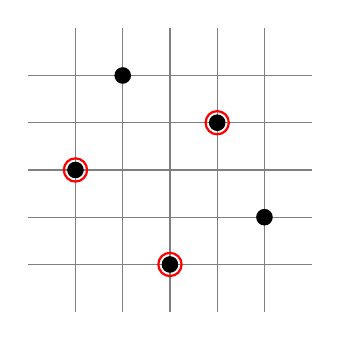
\begin{tikzpicture}[scale=.6, baseline={([yshift=-3pt]current bounding box.center)}]
          \def \n {5}
          \foreach \x in {1,...,\n} {
            \draw[gray] (0,\x) -- (\n+1,\x);
            \draw[gray] (\x,0) -- (\x,\n+1);
          }
          \foreach \x in {(1,3),(2,5),(3,1),(4,4),(5,2)} {\fill[black] \x circle (5pt);}
          \uncover<4->{\foreach \x in {(1,3),(3,1),(4,4)} {\draw[red, thick]  \x circle (7pt);}}
        \end{tikzpicture}
      \end{figure}

      \column{0.6\textwidth}
      \uncover<3->{On the left we have plotted $\Gr{\pi}$ with $\pi = 35142$ from previous examples.\\}
      \uncover<4->{Highlighted with red circles is an occurrence of $\sigma = 213$ in $\pi$.}
    \end{columns}
    \end{example}}
\end{frame}

\begin{frame}{Mesh patterns}
  \uncover<2->{
    \begin{definition}
      A \emph{mesh pattern} is a a pair
      \[p = (\sigma, R) \text{ with } \sigma \in \S_k \text{ and } R \subseteq \llbracket 
      0, k \rrbracket \times \llbracket 0, k \rrbracket \] where $\llbracket 0, k 
      \rrbracket = \{0, 1, \ldots, k\}$ and $R$ is a set of Cartesian coordinates 
      $\boks{i, j}$ denoting the lower left corners of the squares in the grid 
      representation of $\sigma$ which are \emph{shaded}.
    \end{definition}}
  \uncover<3->{
    \begin{example}
    \begin{columns}
      \column{0.35\textwidth}
      \begin{figure}[h]
        \center
        \mpattern{scale=1}{ 3 }{ 1/2, 2/1, 3/3 }{ 1/2, 1/3, 2/2 }
      \end{figure}

      \column{0.6\textwidth}
      The mesh pattern $p = (\sigma, R)$ where $\sigma = 213$ and 
      $R = \left\{ \boks{1,2}, \boks{1,3}, \boks{2,2} \right\}$
      \newline is shown on the left.
    \end{columns}
    \end{example}}
\end{frame}

\begin{frame}{Permutations containing mesh patterns}
\begin{figure}[h]
  \centering
  \raisebox{0.6ex}{%{{{
  \uncover<2->{\shpattb{0.5}{3}{2,1,3}[1/2,2/2,2/3][][][][1/2/2/3, 2/2/3/3, 2/3/3/4]}}
  \quad\quad
  \raisebox{0.6ex}{%{{{
    \uncover<2->{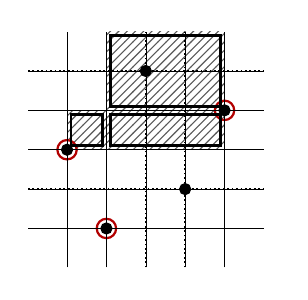
\begin{tikzpicture}[baseline=(current bounding box.center), scale=0.5]
      \useasboundingbox (0.0,-0.1) rectangle (5+1.4,5+1.1);
      \uncover<4->{\foreach \x/\y in {1/3,2/3,2/4,2/5,3/3,3/4,3/5,4/3,4/4,4/5}
        \fill[pattern color = black!65, pattern=north east lines] (\x,\y) rectangle +(1,1);}
      \foreach [count=\x] \y in {3,1,5,2,4}
        \filldraw (\x,\y) circle (4pt);
      \uncover<3->{\foreach \x/\y in {1/3,2/1,5/4}
        \draw[thick,red!70!black] (\x,\y) circle (7pt);}
      
      \draw[very thin] (1,0.01) -- (1,5.99);
      \draw[very thin] (2,0.01) -- (2,5.99);
      \draw[very thin] (5,0.01) -- (5,5.99);
      \draw[very thin] (0.01,1) -- (5.99,1);
      \draw[very thin] (0.01,3) -- (5.99,3);
      \draw[very thin] (0.01,4) -- (5.99,4);

      \uncover<2>{
        \draw[very thin] (3,0.01) -- (3,5.99);
        \draw[very thin] (4,0.01) -- (4,5.99);
        \draw[very thin] (0.01,2) -- (5.99,2);
        \draw[very thin] (0.01,5) -- (5.99,5);
      }
      \uncover<3->{
        \draw[densely dotted, line width=0.6pt] (3,0.01) -- (3,5.99);
        \draw[densely dotted, line width=0.6pt] (4,0.01) -- (4,5.99);
        \draw[densely dotted, line width=0.6pt] (0.01,2) -- (5.99,2);
        \draw[densely dotted, line width=0.6pt] (0.01,5) -- (5.99,5);
      }

      \uncover<4->{\foreach \xa/\ya/\xb/\yb in {1/3/2/4, 2/3/5/4, 2/4/5/6}
        \draw[line width=1pt] (\xa+0.1,\ya+0.1) rectangle (\xb-0.1,\yb-0.1);}
    \end{tikzpicture}}}%}}}
    \quad\quad
    \raisebox{0.6ex}{%{{{
    \uncover<5->{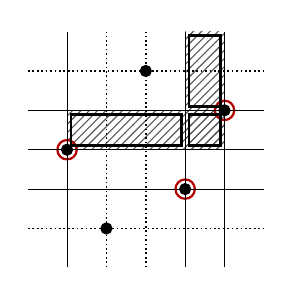
\begin{tikzpicture}[baseline=(current bounding box.center), scale=0.5]
      \useasboundingbox (0.0,-0.1) rectangle (5+1.4,5+1.1);
      \foreach \x/\y in {1/3,2/3,3/3,4/3,4/3,4/4,4/5}
        \fill[pattern color = black!65, pattern=north east lines] (\x,\y) rectangle +(1,1);
      \foreach [count=\x] \y in {3,1,5,2,4}
        \filldraw (\x,\y) circle (4pt);
      \foreach \x/\y in {1/3,4/2,5/4}
        \draw[thick,red!70!black] (\x,\y) circle (7pt);
      
      \draw[very thin] (1,0.01) -- (1,5.99);
      \draw[very thin] (4,0.01) -- (4,5.99);
      \draw[very thin] (5,0.01) -- (5,5.99);
      \draw[very thin] (0.01,2) -- (5.99,2);
      \draw[very thin] (0.01,3) -- (5.99,3);
      \draw[very thin] (0.01,4) -- (5.99,4);

      \draw[densely dotted, line width=0.6pt] (2,0.01) -- (2,5.99);
      \draw[densely dotted, line width=0.6pt] (3,0.01) -- (3,5.99);
      \draw[densely dotted, line width=0.6pt] (0.01,1) -- (5.99,1);
      \draw[densely dotted, line width=0.6pt] (0.01,5) -- (5.99,5);

      \foreach \xa/\ya/\xb/\yb in {1/3/4/4, 4/3/5/4, 4/4/5/6}
        \draw[line width=1pt] (\xa+0.1,\ya+0.1) rectangle (\xb-0.1,\yb-0.1);
    \end{tikzpicture}}}%}}}
    \end{figure}
    \begin{itemize}
      \uncover<2->{\item The mesh pattern $p = \left( 213, \left\{ \boks{1,2}, \boks{2,2}, \boks{2,3} \right\} \right)$ (left)
        and the permutation $\pi = 31524$ (middle).}
      \uncover<3->{\item Even though $314$ (highlighted with red circles) is an occurrence of $213$ in $\pi$} 
        \uncover<4->{this is not an occurrence of $p$ in $\pi$.}
      \uncover<5->{\item However, $p$ is contained in $\pi$ because with the occurrence $324$
        the shaded areas do not overlap with any point in $\pi$.}
      \uncover<6->{\item The set of all permutations that \emph{avoid} the mesh pattern $p$ 
        \newline is denoted with $\Av{p}$.}
    \end{itemize}
\end{frame}

\begin{frame}{Generating functions}
  \uncover<2->{\begin{definition}
    The \emph{generating function (GF)} of the avoidance set $\Av{S}$ is the sum
    \[ \sum_{n = 0}^{+\infty} F_n x^n \] where $F_n = |\Avn{S}|$ for all $n$.
    The \emph{exponential generating function (EGF)} of $\Av{S}$ is the sum
    $\sum_{n = 0}^{+\infty} \frac{F_n}{n!} x^n$.
    We say that the avoidance set is \emph{enumerated} by the GF (or EGF) and that the 
    number sequence $\left( F_n \right)_{n \geq 0}$ is the \emph{enumeration} of $\Av{S}$.
  \end{definition}}
  \uncover<3->{\begin{example}
    The GF of $\Av{21} = \left\{ \epsilon, 1, 12, \ldots \right\}$ is $\sum_{n = 0}^{+\infty} x^n
    = \frac{1}{1 - x}$ so the enumeration is $\left( 1, 1, 1, \ldots \right)$.
    The EGF of $\Av{21}$ is $\sum_{n = 0}^{+\infty} \frac{1}{n!} x^n = e^x$.
  \end{example}}
\end{frame}


%%%%%%%%%%%%%%%%%%%%%%%%%%%%%%%%%%%%%%%%%%%%%%%%%%%%%%%%%%%%%%%%%%%%%%%%%%%%%%%
\subsection{Interesting results}
\begin{frame}{Interesting results}\center{Now we will look at some interesting results obtained with \CombCov.}\end{frame}

\begin{frame}{\emph{Generalized Pattern Avoidance} (2001)}
  One of the papers that we tried replicating results from was the above one by Anders Claesson
  where he studies \emph{generalized permutation patterns} that are specific type of mesh patterns.
  Out of the 6 results in the paper we could replicate 5 of them. Below is one of them.

  \begin{figure}[h]
    \center
      \begin{tabular}{ r c l l }
      $\mc{A} = \Av{ \mpattern{scale=\patttextscale}{ 3 }{ 1/1, 2/2, 3/3 }{ 2/0, 2/1, 2/2, 2/3 } }$ & $=$ & $ 
      \strule{\pattdispscale}{1}{1}{} \mediumsqcup
      \strule{\pattdispscale}{3}{2}{
        (0,1)/$\mc{A}$,
        (1,0)/\point{2pt}, 
        (2,1)/$\mc{B}$
      }$ & $\mc{B} = \Av{ \mpattern{scale=\patttextscale}{ 2 }{ 1/1, 2/2 }{} }$ 
    \end{tabular}
  \end{figure}

  After verifying that the cover is indeed correct it is interesting to derive the
  \emph{exponential generating function (EGF)} $F = \sum_{n \geq 0} \frac{a_n}{n!} x^n$ 
  of the avoidance set and show that $a_n = B_n$, proving that the sequence is enumerated 
  by the Bell numbers.
\end{frame}

\begin{frame}{Deriving the EGF}
  \begin{figure}[h]
    \center
      \begin{tabular}{ r c l l }
      $\mc{A} = \Av{ \mpattern{scale=\patttextscale}{ 3 }{ 1/1, 2/2, 3/3 }{ 2/0, 2/1, 2/2, 2/3 } }$ & $=$ & $ 
      \strule{\pattdispscale}{1}{1}{} \mediumsqcup
      \strule{\pattdispscale}{3}{2}{
        (0,1)/$\mc{A}$,
        (1,0)/\point{2pt}, 
        (2,1)/$\mc{B}$
      }$ & $\mc{B} = \Av{ \mpattern{scale=\patttextscale}{ 2 }{ 1/1, 2/2 }{} }$ 
    \end{tabular}
  \end{figure}

  \begin{itemize}
    \uncover<2->{\item $\mc{A}$ has EGF $F = \sum_{n \geq 0} \frac{a_n}{n!} x^n$}
    \uncover<3->{\item $\mc{B}$ has EGF $\sum_{n \geq 0} \frac{1}{n!} x^n = e^x$}
    \uncover<4->{\item This gives us the recurrence relation $F = 1 + \int F e^x dx$}
    \uncover<5->{\item We solve it and get $F = A e^{e^x}$}
    \uncover<6->{\item Knowing that there is only one permutation of length zero in $\mc{A}$
      we put $a_0 = 1$ into the equation at $x = 0$ and get $A = e^{-1}$}
    \uncover<7->{\item We have now shown that $F = e^{e^x - 1}$ which is indeed \newline the EGF for the Bell numbers.}
  \end{itemize}
\end{frame}

\begin{frame}{\emph{Enumerations of Permutations Simultaneously Avoiding a Vincular and a Covincular Pattern of Length 3} (2017)}
  Paper by C.~Bean, H.~Ulfarsson and A.~Claesson. Out of 40 results we could replicate 11, one of them shown below.

  \begin{figure}[h]
    \centering
    \begin{tabular}{ r c l l }
      $\mc{A} = \Av{ \mpattern{scale=\patttextscale}{ 3 }{ 1/1, 2/2, 3/3 }{ 1/0, 1/1, 1/2, 1/3 }, \mpattern{scale=\patttextscale}{ 3 }{ 1/2, 2/1, 3/3 }{0/2, 1/2, 2/2, 3/2 } }$ & $=$ & $
      \strule{\patttextscale}{1}{1}{} \mediumsqcup
      \strule{\patttextscale}{2}{2}{
        (0,1)/$\mc{A}$, 
        (1,0)/\point{2pt}
      } \mediumsqcup
      \strule{\patttextscale}{4}{4}{
        (0,3)/$\mc{A}$, 
        (1,0)/\point{2pt},
        (2,2)/\point{2pt},
        (3,1)/$\mc{A}$
      } $ &
    \end{tabular}
  \end{figure}

  From this cover it is easy to see that the GF satisfies
  \[ F(x) = 1 + xF(x) + x^2F(x)^2 \]
  which indeed gives us the \emph{Motzkin} numbers $M_n$ to $x^n$ in $F(x)$.
\end{frame}

\begin{frame}{\emph{Wilf-Classification of Mesh Patterns of Short Length} (2015)}
  Paper by Í.~Hilmarsson, I.~Jónsdóttir, S.~Sigurðardóttir, L.~Viðarsdóttir and H.~Ulfarsson.
  Out of 65 results we managed to replicate 15. Some of them shown here without further comments.

  \begin{table}[h]
    \centering
    \begin{tabular}{ r c l l }
      $\Av{ \mpattern{scale=\patttextscale}{ 2 }{ 1/1, 2/2 }{ 0/0, 0/1, 0/2, 1/0, 1/2, 2/0, 2/1 } }$ & $=$ & $
        \strule{\pattdispscale}{1}{1}{} \mediumsqcup
        \strule{\pattdispscale}{2}{2}{
          (0,0)/\point{2pt}, 
          (1,1)/$\mc{B}$
        } \mediumsqcup
        \strule{\pattdispscale}{2}{2}{
          (0,1)/\point{2pt}, 
          (1,0)/\point{2pt},
          (1,1)/$\S$
        }$ & $\mc{B} = \Av{ \mpattern{scale=\patttextscale}{ 1 }{ 1/1 }{ 0/1, 1/0 } }$ \\
    $\Co \left( \mpattern{scale=\patttextscale}{ 2 }{ 1/1, 2/2 }{ 0/0, 0/1, 0/2, 1/0, 1/2, 2/0, 2/1 } \right)$ & $=$ & $
        \strule{\patttextscale}{4}{4}{
          (0,0)/\point{2pt}, 
          (1,1)/$\S$,
          (2,2)/\point{2pt},
          (3,3)/$\mc{B}$
      }$ & 
    \end{tabular}
  \end{table} 
\end{frame}

\begin{frame}
\begin{table}[h]
  \centering
  \begin{tabular}{ r c l l }
    $\Av{ \mpattern{scale=\patttextscale}{ 2 }{ 1/1, 2/2 }{ 0/1, 0/2, 1/0, 1/2, 2/0, 2/1 } }$ & $=$ & $
    \strule{\pattdispscale}{1}{1}{
      (0,0)/$\mc{B}$
    } \mediumsqcup
    \strule{\pattdispscale}{3}{3}{
      (0,0)/$\mc{B}$, 
      (1,1)/\point{2pt},
      (2,2)/$\mc{B}$
    }$ & $\mc{B} = \Av{ \mpattern{scale=\patttextscale}{ 1 }{ 1/1 }{ 0/1, 1/0 } }$ \\
    $\Co \left( \mpattern{scale=\patttextscale}{ 2 }{ 1/1, 2/2 }{ 0/1, 0/2, 1/0, 1/2, 2/0, 2/1 } \right)$ & $=$ & $ 
    \strule{\pattdispscale}{5}{5}{
      (0,0)/$\S$,
      (1,1)/\point{2pt}, 
      (2,2)/$\mc{B}$,
      (3,3)/\point{2pt},
      (4,4)/$\mc{B}$
    }$ &
  \end{tabular}
\end{table} 
\end{frame}

\begin{frame}
\begin{table}[h]
  \centering
  \begin{tabular}{ r c l l }
    $\Co \left( \mpattern{scale=\patttextscale}{ 2 }{ 1/1, 2/2 }{ 0/0, 0/1, 1/1, 1/2, 2/0, 2/2 } \right)$ & $=$ & $
    \strule{\pattdispscale}{5}{5}{
      (0,4)/$\S$, 
      (1,1)/\point{2pt},
      (2,0)/$\S$,
      (3,3)/\point{2pt},
      (4,2)/$\S$
    }$ &
  \end{tabular}
\end{table} 
\end{frame}

\begin{frame}{\emph{Wilf classification of bi-vincular permutation patterns} (2009)}
  Preprint by R.~Parviainen. Out of 24 results we replicated 7.
  \uncover<2->{Below is one of them.} 
  \uncover<3->{It is interesting to compare it to the well known $\Av{132}$.}

  \begin{figure}[h]
    \centering
    \begin{tabular}{ r c l l }
      \uncover<2->{
        $\Av{ \mpattern{scale=\patttextscale}{ 3 }{ 1/1, 2/3, 3/2 }{ 0/3, 1/3, 2/3, 3/3 } }$ & $=$ & $
        \strule{\pattdispscale}{1}{1}{} \mediumsqcup
        \strule{\pattdispscale}{3}{3}{
          (0,1)/$\S$,
          (1,2)/\point{2pt},
          (2,0)/$\S$
        }$ & \\
      }
      \uncover<3->{
        $\mc{A} = \Av{ \mpattern{scale=\patttextscale}{ 3 }{ 1/1, 2/3, 3/2 }{} }$ & $=$ & $
        \strule{\pattdispscale}{1}{1}{} \mediumsqcup
        \strule{\pattdispscale}{3}{3}{
          (0,1)/$\mc{A}$,
          (1,2)/\point{2pt},
          (2,0)/$\mc{A}$
        }$ &
      }
    \end{tabular}
  \end{figure}
\end{frame}


%%%%%%%%%%%%%%%%%%%%%%%%%%%%%%%%%%%%%%%%%%%%%%%%%%%%%%%%%%%%%%%%%%%%%%%%%%%%%%%
\section{Final words}
\begin{frame}{Conclusions}
  \begin{itemize}
    \item We showed that \CombCov\ is a powerful tool in guiding humans by coming up with 
      conjectures that would otherwise have required substantial effort to discover manually.
    \item We were pleasantly surprised in how many published results it found covers for.
    \item \CombCov's shortcomings may be remedied with improved ways of coming up with and 
      generate the rules.
  \end{itemize}
\end{frame}

\begin{frame}{Any questions?}
  \center{\Large{``There is no such thing as a dumb question.''}}
  \\[5pt]
  \rightline{{\rm --- Carl Sagan}} 
\end{frame}

\end{document}
